\documentclass[12pt,titlepage]{article}

\usepackage[T1]{fontenc}
\usepackage[utf8]{inputenc}
\usepackage[french]{babel} 
\usepackage[top=1.5cm, bottom=1.5cm, left=1.5cm, right=1.5cm]{geometry}
\usepackage{multicol}
\usepackage{lipsum}
\usepackage{ragged2e}
\usepackage{eurosym}
\usepackage{indentfirst}
\usepackage{titlesec}
\usepackage{pifont}
\usepackage{epsf}

%------- TXT --------
\usepackage{enumerate}
\usepackage{xcolor}
%------- WEB --------
\usepackage{url}
\usepackage[colorlinks=true, allcolors=blue]{hyperref}
%------- MATH --------
\usepackage{amsmath}
\usepackage{amsfonts}
\usepackage{amssymb}
%------- GRAPH -------
\usepackage{graphicx}
\usepackage{float}
\usepackage{wrapfig}
\usepackage{caption}
\usepackage{subcaption}
%------ CODE ---------
\usepackage{minted}

\graphicspath{ {./image/} }
\newcommand{\HRule}{\rule{\linewidth}{0.5mm}}


\begin{document}

\begin{titlepage}

\begin{center}
    
\includegraphics[scale = 0.35]{uliege_facsa.jpg}\\
    
    \vspace{1cm}
    
    \textsc{\huge Université de Liège}\\[1.2cm]
    
    \HRule \\[1cm]
    
    \textsc{\LARGE Introduction to machine learning (ELEN062-1) }\\[1cm]
    
    {\Huge \bfseries Projet 2 : Bias and variance analysis }\\[1.4cm] 
    
    \HRule \\[1cm]
    
\end{center}

\begin{minipage}{0.45\linewidth}
      \begin{flushleft} \large
      
        \emph{Authors : } \\
        Louis \textsc{HOGGE}  s192814\\
        Simon \textsc{LOUVEAU}  s194100\\
        Tom \textsc{WEBER}  s203806
        
      \end{flushleft}
\end{minipage}
\hfill
\begin{minipage}{0.45\linewidth}
      \begin{flushright} \large
      
        \emph{Professor : } L. \textsc{Wehenkel}\\
        \emph{Professor : } P. \textsc{Geurts}\\
        \emph{Year : } 2023-2024 
        
      \end{flushright}
\end{minipage}

\end{titlepage}

\section{Anatical derivation}

\subsection{Analytical expression}

Data of the ridge regression problem :
\begin{enumerate}
    \item[$\bullet$] Learning sample of N pairs, $LS = \{(x_{1}, y_{1}), ..., (x_{N}, y_{N})\}$ with $(x_{i}, y_{i}) \in \mathbb{R} x \mathbb{R}$
    \item[$\bullet$] Values of input variables $x_{i}$ are fixed while ouput variables are $y_{i} = wx_{i} + \epsilon_{i}$, where $e_{i}$'s are independent and identically drawn from a normal distribution $\mathcal{N}(0, \sigma^{2})$.
    \item[$\bullet$] $\hat{w}_{LS} = \arg \min_{w'}\{\sum_{i=1}^{N}(y_{i}-w'x_{i})^{2}+\lambda w'^{2}\}$, with $\lambda \geq 0$ the regularization hyper-parameter
    \item[$\bullet$] w' is the weight we want to estimate
    \item[$\bullet$] Let us call the cost function F(w') such that $F(w') = \sum_{i=0}^{N} (y_{i}-w'x_{i})^{2} + \lambda w'^{2}$
    \item[$\bullet$] $x_{0}$ will be referring to a specific test point.
    \item[$\bullet$] $s_{xx} = \sum_{i}x_{i}^{2}$ and $s_{xy} = \sum_{i} x_{i}y_{i}$
\end{enumerate}
Now, analytical expressions are given with explainations here-under.
\begin{enumerate}
    \item[1.] $\hat{w}_{LS}$ \\
    To find the $\hat{w}_{LS}$ that minimizes the cost function F(w') defined in the preamble, we take the derivative of F(w') with respect to w', set it to zero and solve for w'.\\
    Taking the derivative : $$ \frac{d F(w')}{dw'} = \frac{d}{dw'}(\sum_{i=1}^{N}(y_{i}-w'x_{i})^{2} + \lambda w'^{2})$$
    Expanding the derivative : $$ = \sum_{i=1}^{N} 2(y_{i}-w'x_{i})(-x_{i}) + 2 \lambda w' $$
    $$ = -2 \sum_{i=1}^{N}x_{i}y_{i} + 2w'\sum_{i=1}^{N}x_{i}^{2} + 2 \lambda w' $$
    Setting this derivative equal to zero to find the minimium : $$ -2 \sum_{i=1}^{N}x_{i}y_{i} + 2w'\sum_{i=1}^{N}x_{i}^{2} + 2 \lambda w' = 0 $$
    Simplifying and solving for w' : 
    $$ w'(\sum_{i=1}^{N}x_{i}^{2} + \lambda) = \sum_{i=1}^{N}x_{i}y_{i} $$
    $$ w' = \frac{\sum_{i=1}^{N}x_{i}y_{i}}{\sum_{i=1}^{N}x_{i}^{2} + \lambda} = \hat{w}_{LS} = \frac{s_{xy}}{s_{xx} + \lambda}$$
    \item[2.] Bayes model, $h_{B}(x_{0})$ \\
    To find $h_{B}(x_{0})$, the model that predicts the expected value of y given x is to be determined, using the distribution of y conditioned on x. In our case, $y = wx + \epsilon$, where $\epsilon$ is normally distributed as $\mathcal{N}(0,\sigma^{2})$. The Bayes model, $h_{B}(x)$, is the model that minimizes the expected prediction error for a new input x, which in the case of regression is typically the expected value of y given x. Given that $\epsilon$ is normally distributed with mean 0, the expected value of y given x simplifies to the deterministic part of the relationship as $E\{\epsilon\} = 0$ as $\epsilon$ is from a $\mathcal{N}(0, \sigma^{2})$.\\
    Therefore, the Bayes model, $h_{B}(x_{0})$ for a new input $x_{0}$ in this case is $h_{B}(x_{0}) = E\{y|x=x_{0}\} = wx_{0}$. \\
    $h_{B}(x_{0})$ represents the theoretical best prediction under the given model of data.
     \item[3.] Residual error, $noise(x_{0})$ \\
     The residual error in a regression context typically refers to the difference between the observed values and the predicted values.
     As seen from the theoretical notes, $noise(x_{0}) = E_{y|x_{0}}\{(y-h_{B}(x_{0}))^{2}\}$ quantifies how much y varies from $h_{B}(x_{0}) = E_{y|x_{0}}\{y\}$ (Bayes model).
     We know that $y = wx + \epsilon$ where $\epsilon$ is the only source of randomness in the learning sample and drawn from a normal distribution $\mathcal{N}(O, \sigma^{2})$ meaning its expectation is 0 (will be used when simplifying expressions). Thus, the analytical expression simply becomes :  
     $$noise(x_{0}) =  E_{y|x_{0}}\{((wx_{0} + \epsilon))-wx_{0})^{2}\} =  E_{y|x_{0}}\{\epsilon^{2}\} = noise(x_{0})$$
     We know in general that for any random variable X, $Var\{X\} = E\{X^{2}\} - E\{X\}^{2}$. So, in our case, $$E_{y|x_{0}}\{\epsilon^{2}\} = Var\{\epsilon\} + E\{\epsilon\}^{2} = Var\{\epsilon\} = \sigma^{2}$$
    \item[4.] Squared bias, $bias^{2}(x_{0})$ \\
    Bias measures the error between the Bayes model and the average model. \\
    It is given by $bias^{2}(x_{0}) = (h_{B}(x_{0}) - E_{LS}\{\hat{y}(x_{0})\})^{2}$
    In our case, the true value of the model is given by $y = wx + \epsilon$ where $\epsilon$ is normally distributed with a mean of 0. The Bayes model $h_{B}(x) = wx$ and for the ridge regression, the prediction at $x_{0}$ is given by $\hat{y}(x_{0}) = \hat{w}_{LS}x_{0}$ where $\hat{w}_{LS}$ is the estimate for the weight w using the ridge regression. \\ Thus,
    $$ bias^{2}(x_{0}) = (h_{B}(x_0) - E_{LS}\{\hat{y}(x_{0})\})^{2} $$
    Given that $E_{LS}\{\hat{y}(x_{0})\}$ is $E_{LS}\{\hat{w}_{LS}\}x_{0}$ as as $E\{\epsilon\} = 0$ and $h_{B}(x_{0})$ is $wx_{0}$, the expression becomes : $$ bias^{2}(x_{0}) = (wx_{0}-E_{LS}\{\hat{w}_{LS}\}x_{0})^{2}$$
    In addition, the expectation with respect to $\epsilon_{i}$ is considered as $x_{i}$ are fixed and w, $\lambda$ are constants, and we can substitute $y_{i} = wx_{i}+\epsilon_{i}$, so we have $$ E_{LS}\{\hat{w}_{LS}\} = E_{LS}\left\{\frac{\sum_{i=1}^{N}x_{i}y_{i}}{\sum_{i=1}^{N}x_{i}^{2} + \lambda}\right\} = E_{LS}\left\{\frac{\sum_{i=1}^{N}x_{i}(wx_{i}+\epsilon_{i})}{\sum_{i=1}^{N}x_{i}^{2} + \lambda}\right\} = E_{LS}\left\{\frac{w\sum_{i=1}^{N}x_{i}^{2} + \sum_{i=1}^{N} x_{i}\epsilon_{i}}{\sum_{i=1}^{N}x_{i}^{2} + \lambda}\right\} $$
    But since $\sum_{i=1}^{N} x_{i}^{2}$ and $\lambda$ are constants, they come out of the expectation and the expectation of the sum involving $\epsilon_{i}$ is zero, we have $$E_{LS}\{\hat{w}_{LS}\} = \frac{w\sum_{i=1}^{N}x_{i}^{2}}{\sum_{i=1}^{N}x_{i}^{2} + \lambda} = \frac{w s_{xx}}{s_{xx} + \lambda}$$
    $$ bias^{2}(x_{0}) = (wx_{0}-E_{LS}\{\hat{w}_{LS}\}x_{0})^{2} = (wx_{0}-\frac{w s_{xx}}{s_{xx} + \lambda} x_{0})^{2}$$
    This can be even more simplified by and it is as follows
    $$ bias^{2}(x_{0}) =\left(\frac{w x_{0} \lambda}{s_{xx} + \lambda}\right)^{2}$$
    \item[5.] Variance, $variance(x_{0})$ \\
    The $variance(x_{0})$ quantifies how much the average over the whole input space varies from one learning sample to another. In our ridge regression model, the prediction for a given input $x_{0}$ is : $\hat{y}(x_{0}) = \hat{w}_{LS}x_{0}$.
    Furthermore, the variance is concerned with how much $\hat{y}(x_{0})$ varies as the training data varies while $x_{0}$ remains fixed ! This variance is due to the randomness in the training data particularly the noise terms $\epsilon_{i}$. Variance of the prediction at $x_{0}$ is :
    $$ variance(x_{0}) = E_{LS}[(\hat{y}(x_{0})-E_{LS}[\hat{y}(x_{0})])^{2}] $$
    Since $E[\hat{y}(x_{0})]$ is $E[\hat{w}_{LS}]x_{0}$, we have :
    $$ variance(x_{0}) = E_{LS}[(\hat{w}_{LS}x_{0} - E[\hat{w}_{LS}]x_{0})^{2}] $$
    which simplifies with the help of above results to :
    $$ variance(x_{0}) = E_{LS}[(\hat{w}_{LS}x_{0} - \frac{ws_{xy}}{s_{xx} + \lambda}x_{0})^{2}]$$
    By using the general rules $Var(cX) = c^{2}Var(X)$ and afterwards $E(x^{2}) = Var(X) + E(X)^{2})$, we get 
    $$ variance(x_{0}) = x_{0}^{2} E_{LS} \left\{ (\hat{w}_{LS} - \frac{w s_{xx}}{s_{xx} + \lambda})^{2} \right\}$$
    $$ variance(x_{0}) = x_{0}^{2} \left(Var\{\hat{w}_{LS} - \frac{w s_{xx}}{s_{xx} + \lambda}\} + E_{LS} \left\{\hat{w}_{LS} - \frac{w s_{xx}}{s_{xx} + \lambda}\right\}^{2}\right)$$
    The fact that $\frac{w s_{xx}}{s_{xx} + \lambda}$ is a constant allows the simplification using the general rule $Var(X + c) = Var(X)$ as follows
    $$ variance(x_{0}) = x_{0}^{2} \left(Var\{\hat{w}_{LS}\} + E_{LS} \left\{\hat{w}_{LS} - \frac{w s_{xx}}{s_{xx} + \lambda}\right\}^{2}\right)$$
    By using $E(X^{2}) - Var(X) = E(X)^{2}$, we get
    $$ variance(x_{0}) = x_{0}^{2} \left(Var\{\hat{w}_{LS}\} + E_{LS} \left\{\left(\hat{w}_{LS} - \frac{w s_{xx}}{s_{xx} + \lambda}\right)^{2} \right\} - Var\{\hat{w}_{LS} - \frac{w s_{xx}}{s_{xx} + \lambda}\} \right) $$
    Using again the general rule $Var(X + c) = Var(X)$, we have
    $$ variance(x_{0}) = x_{0}^{2} \left(Var\{\hat{w}_{LS}\} + E_{LS} \left\{\left(\hat{w}_{LS} - \frac{w s_{xx}}{s_{xx} + \lambda}\right)^{2} \right\} - Var\{\hat{w}_{LS}\} \right) $$
    Which gives us 
    $$ variance(x_{0}) = x_{0}^{2} E_{LS} \left\{\left(\hat{w}_{LS} - \frac{w s_{xx}}{s_{xx} + \lambda}\right)^{2} \right\} $$
    By expanding the square, we obtain
    $$ variance(x_{0}) = x_{0}^{2} E_{LS} \left\{\hat{w}_{LS}^{2} - \frac{2 w s_{xx} \hat{w}_{LS}}{s_{xx} + \lambda} + \frac{w^{2} s_{xx}^{2}}{(s_{xx} + \lambda)^{2}} \right\} $$
    Again, this simplifies to
    $$ variance(x_{0}) = x_{0}^{2} \left\{ E_{LS} \left\{\hat{w}_{LS}^{2}\right\} - \frac{2 w s_{xx}}{s_{xx} + \lambda}E_{LS} \left\{\hat{w}_{LS}\right\} + \frac{w^{2} s_{xx}^{2}}{(s_{xx} + \lambda)^{2}} \right\} $$
    Since $E_{LS}\{\hat{w}_{LS}\} = \frac{w s_{xx}}{s_{xx} + \lambda}$, we have
    $$ variance(x_{0}) = x_{0}^{2} \left\{ E_{LS} \left\{\hat{w}_{LS}^{2}\right\} - 2w^{2}\left(\frac{s_{xx}}{s_{xx} + \lambda}\right)^{2}  + \frac{w^{2} s_{xx}^{2}}{(s_{xx} + \lambda)^{2}} \right\} $$
    Let's consider the $E_{LS} \left\{ \hat{w}_{LS}^{2} \right\}$,
    $$ E_{LS} \left\{ \hat{w}_{LS}^{2} \right\} = E_{LS} \left\{ \hat{w}_{LS} \right\}^{2} + Var\{\hat{w}_{LS}\} = \left( \frac{w s_{xx}}{s_{xx} + \lambda} \right)^{2} + Var\{\hat{w}_{LS}\}$$
    Putting back the value into the equation of the variance we found gives us
    $$ variance(x_{0}) = x_{0}^{2} \left\{ \left( \frac{w s_{xx}}{s_{xx} + \lambda} \right)^{2} + Var\{\hat{w}_{LS}\} - 2w^{2}\left(\frac{s_{xx}}{s_{xx} + \lambda}\right)^{2}  + \frac{w^{2} s_{xx}^{2}}{(s_{xx} + \lambda)^{2}} \right\} $$
    Which simplifies to
    $$ variance(x_{0}) = x_{0}^{2} \left\{ Var\{\hat{w}_{LS}\} \right\} $$
    Let's consider $Var\{\hat{w}_{LS}\}$, knowing that the variance of a constant is zero, thet $e_{i}$ have a variance of $\sigma^{2}$ by definition and that $Var(cX) = c^{2} Var(X)$,
    $$ Var\{\hat{w}_{LS}\} = Var \left\{ \frac{w \sum_{i=1}^{N} x_{i}^{2} + \sum_{i=1}^{N} x_{i} \epsilon_{i}}{\sum_{i=1}^{N} x_{i}^{2} + \lambda} \right\} = \frac{\sum_{i=0}^{N} x_{i}^{2}}{(s_{xx} + \lambda)^{2}} Var(e_{i}) = \frac{\sum_{i=0}^{N} x_{i}^{2}}{(s_{xx} + \lambda)^{2}} \sigma^{2}$$
    Thus, the final expression of the variance is 
    $$ variance(x_{0}) = x_{0}^{2} \frac{\sum_{i=0}^{N} x_{i}^{2}}{(s_{xx} + \lambda)^{2}} \sigma^{2} $$
    $$ variance(x_{0}) = x_{0}^{2} \sigma^{2} \frac{s_{xx}}{(s_{xx} + \lambda)^{2}} $$
    
\end{enumerate}

\subsection{Impact of paramaters on bias and variance}
Now let us discuss the impact of the following parameters on both bias and variance. \\
Recall that $\hat{w}_{LS} = \frac{s_{xy}}{s_{xx} + \lambda}$, $bias^{2}(x_{0}) =\left(\frac{w x_{0} \lambda}{s_{xx} + \lambda}\right)^{2}$ and $variance(x_{0}) = x_{0}^{2} \sigma^{2} \frac{s_{xx}}{(s_{xx} + \lambda)^{2}}$
\begin{enumerate}[a.]
    \item 
    \textbf{Regularization level} $\lambda$ \\
    $\lambda$ is a non-negative parameter so it makes sense to understand how bias and variance act when $\lambda$ tends towards $+\infty$ or 0.
    \begin{itemize}
        \item[I.] $\lambda \rightarrow +\infty$ \\
        \begin{itemize}
            \item[A.] Bias \\
            In the limit, the bias term approaches $wx_{0}$ and $bias^{2}$ approaches $wx_{0}^{2}$ which becomes large if w and $x_{0}$ are non-zero.
            \item[B.] Variance \\
            The variance approaches zero as $\lambda$ grows because the denominator grows much faster than the numerator. Thus, a very large $\lambda$ allows model's prediction to become very stable with low variance but at the cost of a high bias if true weights are not near zero.
        \end{itemize}
        \item[II.] $\lambda \rightarrow 0$ \\
        \begin{itemize}
            \item[A.] Bias \\
            bias is 0. The ridge estimator is unbiased and this is typical to the classical least squares estimator. 
            \item[B.] Variance \\
            Variance becomes $ \frac{x_{0}^{2}\sigma^{2}}{s_{xx}}$. There is no regularization to constrain the weights. This can lead to high variance.
        \end{itemize}
        \item[III.] Discussion \\
        It seems that in the context of the ridge regression, the $\lambda$ parameter has a high impact on multiple aspects. First, when $\lambda$ is too small, overfitting occurs as the model is too complex. There is no regularization so the model may fit the training data very well but it will likely perform poorly on the unseen data because of its low bias and high variance. \\
        Then, when $\lambda$ is too large, it can lead to underfitting. Underfitting is caused by the shrinkage of coefficients (coefficients tends to become so small due to the optimization of the cost function that they may approach zero resulting in a model that is too simple and doesn't fit the training data). \\
        In addition to this, there is a clear bias-variance trade-off as increasing $\lambda$ introduces bias with a significant reduction in variance and conversely when $\lambda$ is decreasing.
    \end{itemize}
    \item 
    \textbf{Noise} $\sigma$ \\
    \begin{itemize}
        \item[I.] Bias \\
        The bias doesn't depend on $\sigma$ as can be seen by looking at its expression. So, $\sigma$ has no effect on the bias.
        \item[II.] Variance \\
        Variance is directly proportional to $\sigma^{2}$.
        \begin{itemize}
            \item[A.] $\sigma \rightarrow +\infty$ \\
            As $\sigma$ increases, variance increases with no bound.
            \item[B.] $\lambda \rightarrow +0$ \\
            As $\sigma$ decreases, so does the variance.
        \end{itemize}
        \item[III.] Discussion \\
        As $\sigma$ increases, so does the variances, bringing more noise. Thus, the model's predictions are less reliable with higher uncertainty.
    \end{itemize}
    \item 
    \textbf{Learning sample size} $N$ \\
    Following the suggestion, $x_{i}$ are assumed to have been drawn from a normal distribution $\mathcal{N}(0,1)$. We know that $s_{xx}$ is defined as 
    $$ s_{xx} = \sum_{i=1}^{N} x_{i}^{2}$$
    Each $x_{i}^{2}$ is a random variable that follows a chi-squared distribution with degree 1 of freedom because it is the square of a standard variable following the normal distribution as assumed by the suggestion. The expectation of such variable is its degree of freedom which in our case is 1. Therefore, $$ E\{ x_{i}^{2} = 1 \} $$
    For a large number of $x_{i}$, by the law of large numbers, the average of the $x_{i}^{2}$'s will converge to the expected value of a single $x_{i}^{2}$ as N tends to $+\infty$. As a reminder, the law of large numbers states that as the size of the sample increases, the sample mean (in our cas, sample mean of $x_{i}^{2}$) will converge to the expected value of the population mean. This means 
    $$ \frac{s_{xx}}{N} = \frac{1}{N} \sum_{i=1}^{N}x_{i}^{2} \approx E\{ x_{i}^{2} = 1 \}$$
    $$ s_{xx} \approx N $$
    The larger the N, the closer $s_{xx}$ will be equal to N. \\
    With that in mind we can then analyse how will the bias and variance be influenced by N. \\
    \begin{itemize}
        \item[A.] Bias \\
        $$ bias^{2}(x_{0}) =\left(\frac{w x_{0} \lambda}{s_{xx} + \lambda}\right)^{2} $$
        If N increases, $s_{xx}$ increases, thus $s_{xx} + \lambda$ increases too resulting in a smaller ratio $\frac{\lambda}{s_{xx} + \lambda}$ meaning a smaller bias.
        \item[B.] Variance \\
        $$variance(x_{0}) = x_{0}^{2} \sigma^{2} \frac{s_{xx}}{(s_{xx} + \lambda)^{2}}$$
        Numerator is directly proportional to N but the denominator increases faster as N grows so the expression will decrease as N grows.
        \item[C.] Discussion \\
        As N increases, both bias and variance decreases. This shows that model's predictions are becoming more consistent across different samples.
    \end{itemize}
\end{enumerate}

\subsection{Analytical expression of $\lambda_*$}

The goal of the following section is to derive an analytical expression of the optimal value of $\lambda_*$, i.e. the value of $\lambda$ that leads to the smallest expected generalization error. \\
% Theoretical lecture 6 : 19/95
As seen from the theoretical lecture, the expected generalized error is given by 
$$ E = var_{y}\{y\} + bias^{2} + var_{LS}\{\hat{y}\} $$
Which in our case becomes 
$$ E(x_{0}) = Var_{y}\{y(x_{0})\} + bias^{2}(x_{0}) + Var_{LS}\{\hat{y}(x_{0})\} $$ 
where we replace $x_{0}$, the test point, by $\lambda$.\\
This expression contains :
\begin{itemize}
    \item[1.] $Var_{y}\{y(x_{0})\}$ is the irreducible error
    \item[2.] $bias^{2}(x_{0})$ is the squared bias
    \item[3.] $Var_{LS}\{\hat{y}(x_{0})\}$ is the variance of the model's predictions in the learning sample
\end{itemize}
Given that only the squared bias and the variance of the model's predictions in the learning sample depend on $\lambda$, to find the optimal $\lambda$, $\lambda^{*}$, we need to minimize the sum of the squared bias and the mentioned variance. To do so, We take the derivative of $E(\lambda)$ with respect to $\lambda$ and we equal it to 0. Solving for $\lambda$ gives $\lambda^{*}$. Therefore
$$ \frac{\partial E(\lambda)}{\partial \lambda} = 0 $$
$$ \frac{\partial}{\partial \lambda}\left(\left(\frac{wx_{0}\lambda}{s_{xx} + \lambda}\right)^{2} + \frac{x_{0}^{2}\sigma^{2}s_{xx}}{(s_{xx} + \lambda)^{2}}\right) = 0$$

%%%%%%%%%%%%%%%%%%%%%
% Using a solver
% https://www.wolframalpha.com/input?i2d=true&i=Partial%5B%5C%2840%29Power%5B%5C%2840%29Divide%5Bw+x+%CE%B1%2Cs+%2B+%CE%B1%5D%5C%2841%29%2C2%5D%2B+Divide%5BPower%5Bx%2C2%5DPower%5B%CF%83%2C2%5Ds%2CPower%5B%5C%2840%29s+%2B+%CE%B1%5C%2841%29%2C2%5D%5D%5C%2841%29%2C%CE%B1%5D%3D+0
%%%%%%%%%%%%%%%%%%%%%

$$ \frac{2 \lambda s_{xx} w^2 x_{0}^2}{\lambda^3 + s_{xx}^3 + 3 \lambda s_{xx}^2 + 3 \lambda^2 s_{xx}} - \frac{2 s_{xx} \sigma^2 x_{0}^2}{\lambda^3 + s_{xx}^3 + 3 \lambda s_{xx}^2 + 3 \lambda^2 s_{xx}} = 0 $$

$$ \frac{2 \lambda s_{xx} w^2 x_{0}^2}{(\lambda + s_{xx})^{3}} - \frac{2 s_{xx} \sigma^2 x_{0}^2}{(\lambda + s_{xx})^{3}} = 0 $$

Solving this for $\lambda$ gives
$$ \lambda^{*} = \frac{\sigma^{2}}{w^{2}}$$

In order to discuss the expression, we can consider two things : 
\begin{itemize}
    \item[1.] The numerator $\sigma^{2}$ \\
    This is the noise. If the noise is high, it would need a higher value of $\lambda$ to prevent overfitting.
    \item[2.] The denominator $w^{2}$ \\
    This is the true weight also referenced as the signal.
\end{itemize}

The optimization process for finding $\lambda^{2}$ finally showed that $\lambda^{2}$ is inversely proportional to the well known signal-to-noise ratio but applied in the context of the ridge regression. We can adapt the traditional way of thinking to this new "noise-to-signal" ratio. A high "noise-to-signal" ratio calls for more regularization to prevent
 the model from learning noise as if it were a true signal. Conversely, a low "noise-to-signal" ratio means the true underlying pattern is clear and the model doesn't need as much regularization to make accurate predictions.
 
%%%%%%%%%%%%%%%%%%%%%%%%%%%%%%%%%%%%%%%%%%%%%%%%%%%

\section{Empirical analysis}

\subsection{Residual error estimation}

Let’s start by observing that estimating the residual error will be quite hard in this setting. \\

The residual error is represented as $var_{y \mid x}(y)$, which is difficult to estimate because it’s a variance calculated at specific input points. Given that our dataset is finite and consists of continuous values, it’s highly improbable to have a significant number of outputs for the same input. Since our learning set has a high dimension makes it even more unlikely. In the vast majority of cases, we’ll have a unique output for each input, which makes the computation of $var_{y \mid x}(y)$ excessively difficult.

\subsection{Estimation protocol}
Protocol to estimate variance, the expected error and the sum of the bias and the residual error in few steps.

\begin{enumerate}
    \item 
    Create Learning Sample: \\ 
    We decide to take the same separation ratio as the previous project, so 80\% of it to create 50 random training sets (shuffled from the big training set) of size 500 (size for next question) and 20\% to test the model.

    \item 
    Fit the model to the learning samples and test it on the test set.

    \item 
    Compute the expected error: \\
    Take the mean of the squares of the differences between all true values of output and the outputs which is computed with the model. Then compute the mean of this value over all 50 learning samples.
    \[ 
    E_{LS}\Bigl\{ 
    E_{y \mid \underline{x}} 
    \{ (y - \hat{y}(\underline{x}))^{2} \} 
    \Bigr\} 
    \]

    \item 
    Compute the variance: \\
    Compute the mean over all learning samples of the squares of the differences between the predicted values and the mean of the predicted values.
    \[ 
    E_{LS}\Bigl\{ 
    \left(
    \hat{y}(\underline{x}) - E_{LS} \{ \hat{y}(\underline{x}) \}
    \right)^{2} 
    \Bigr\} 
    \]

    \item 
    Compute the sum of the squared bias and the residual error: \\
    Simply subtract the variance from the expected error.

    \[
    \text{noise}(\bar{x}) + \text{bias}^2(\bar{x}) = 
    E_{LS}
    \Bigl\{ 
    E_{y \mid \underline{x}} 
    \{ (y - \hat{y}(\underline{x}))^{2} \} 
    \Bigr\}  -
    \text{Var}(\underline{x})
    \]
    
\end{enumerate}

\subsection{Impact of the complexity on bias and variance}
For all three models, we observe the impact of their complexity (related to the value of their respective hyper-parameter: $\alpha, k, max\_depth$) on the expected error, the variance and the bias. 

Generally, we should observe an increase in variance and a drop of bias as the complexity of the model increases.
Indeed, as the model gets more and more complex, it starts to better fit our learning data which leads to more possible outputs for each inputs of the test set and thus a higher variance. \\
As the complexity increases, the mean output of the model also gets closer to the real one which leads to a lower bias. On the other hand, as a model gets simpler, the bias gets bigger and bigger (and the variance gets smaller). 

\vspace{0.2cm}

- Overfitting: \\
At some point, it might even start fitting the noise in our data which will significantly increase the error of the model.

\vspace{0.2cm}

- Underfitting: \\
At some point, the model can even become too simple. The corresponding increase in bias will then significantly increase the error and prevent the model from being accurate.

$\Rightarrow$ underfitting and overfitting are bad to the generalization error of the model.

\vspace{0.3cm}

Since the expected error is the sum of the bias and the variance, it is expected to first decrease with the decrease of bias and then increase because of the variance.

\vspace{0.3cm}

The bias-variance tradeoff is the fact we cannot decrease as much as wanted the bias and the variance at the same time.

\subsubsection{Ridge regression}
For the ridge model, it’s important to understand that high values of $\alpha$ means low complexity of the model. \\

Ridge regression is a modified version of the classic regression algorithm. Instead of minimizing the residual sum of squares ($RSS$), it wants to add the product of $\alpha$ by the sum of the squared coefficient to this loss function. It will allow ridge regression to
penalize large coefficients $\xi$.

\[ \sum_{i=1}^{N}(y_i - \hat{y}_i)^2 + \alpha \sum_{j=1}^{M} \xi_{j}^{2} \quad \alpha \in [0 ; \infty] \]

\label{eq:loss_fct}

Minimizing this loss function is equivalent to this:

\[ \text{argmin}(RSS) \rightarrow \sum_{j=1}^{M} \xi_{j}^{2} < \frac{1}{\alpha} \]

With equation above and the Figure \ref{fig:error_ridge}: \\
\begin{itemize}
    \item 
    For small complexity (larger $\alpha$ gets), the smaller the sum of the square of the coefficient must be in order to be selected to minimize the loss function. They (the $\xi$’s) can less vary in the values they can take. This induces less variability and a higher bias.
    
    \item 
    For high complexity ($\alpha$ gets really small), the $\xi$’s can take more possible values to possibly take which directly leads to higher variance and lower bias.
\end{itemize}


\begin{figure}[H]
    \centering
    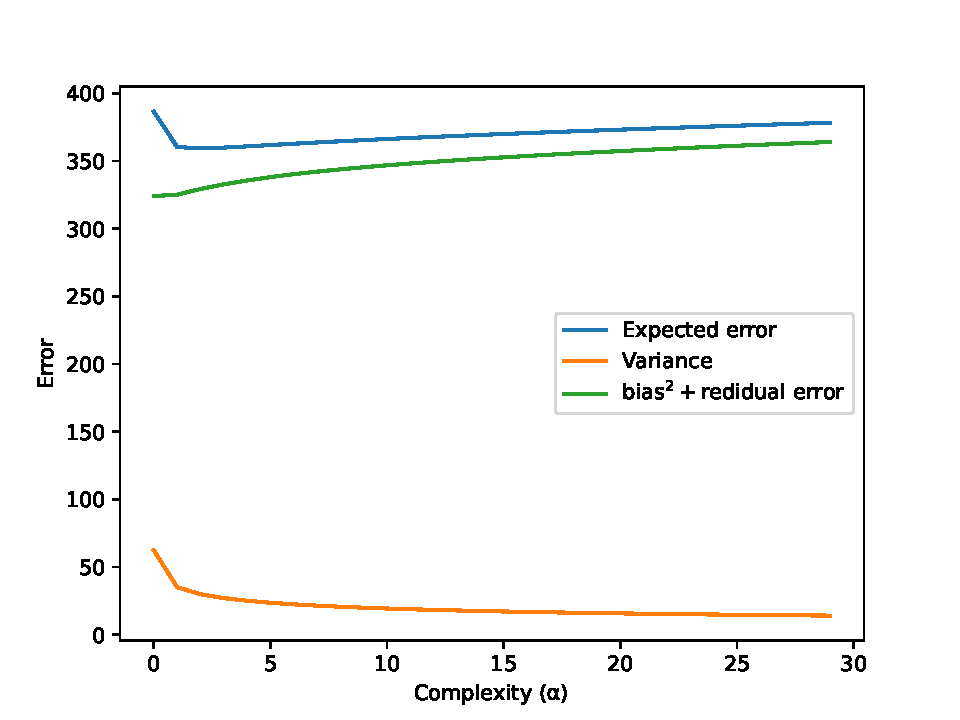
\includegraphics[scale = 0.8]{image/2.3_ridge_regressor.pdf}
    \caption{Error of Ridge regression related to complexity}
    \label{fig:error_ridge}
\end{figure}

\subsubsection{k-NN}
For the k-NN model, k represents the number of neighbours taken into account in order to make
predictions. \\
- If $k$ is small, the model will get extremely complex in order to correctly predict every value given in the learning set (sensitive to noise), leading to high variance and low bias. Case of overfitting \\
- If $k$ increases, the model becomes less complex and its predictions become more stable, but it may start to underfit, leading to higher bias and lower variance. \\
- If $k$ is the total number of inputs in the learning set, this model yields the same value for any input from the test set, the variance in such an extreme case is not zero because it depends on the learning set (it will reach some constant)


\begin{figure}[H]
    \centering
    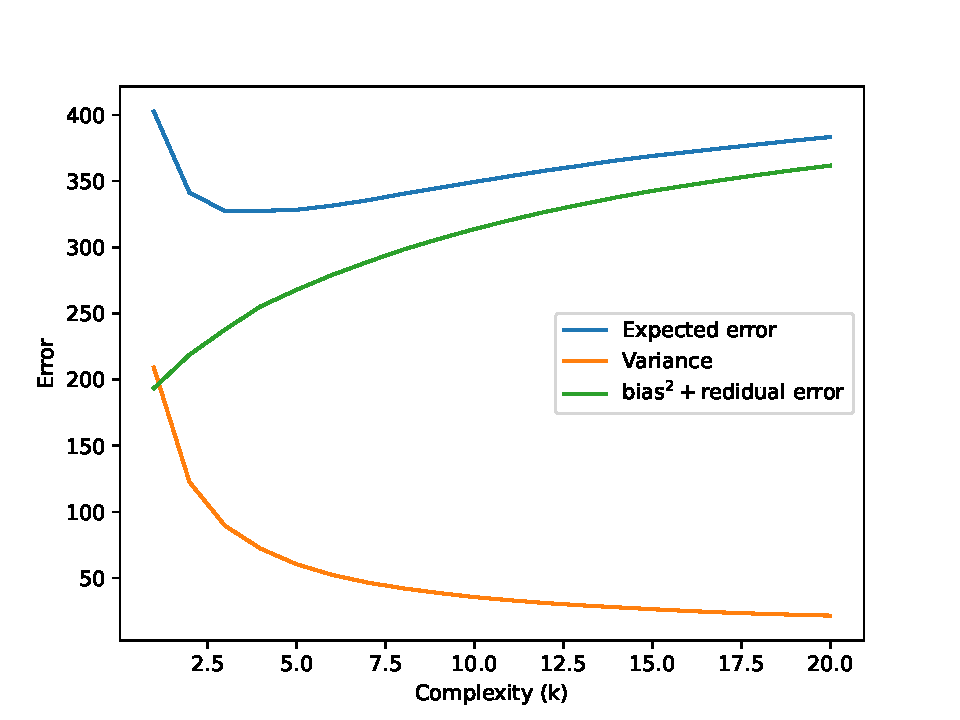
\includegraphics[scale = 0.8]{image/2.3_knn_regressor.pdf}
    \caption{Error of k-NN related to complexity}
    \label{fig:error_knn}
\end{figure}

\subsubsection{Regression trees}
For the regression tree, the maximal
depth of the tree is a measure of the complexity of the model.

Observation made in Figure:\ref{fig:error_dt}:

\begin{itemize}
    \item 
    For very low complexity (very low depth), the bias dominates the variance. The model is underfitting and the error is important. For example, with a maximum depth of only 1, the tree makes a single separation in the learning set and cannot include details that the learning set may have such as a more complex curve that cannot be approximated by a single line (low complexity).

    \item 
    When increasing the depth of the tree (tends towards a fully grown tree), the variance increases and the model starts to overfit. This leads to a smaller bias but an increasing error. If we use, the maximal depth that will allow to perfectly predict the learning set up to the smallest detail (high complexity), it will not predict the outputs of the test set very well because the noise of the learning sample is fit by the mode.
\end{itemize}

\vspace{0.3cm}

$\Rightarrow$ In this model, the complexity does not need to be high to obtain less error and a better bias.

\begin{figure}[H]
    \centering
    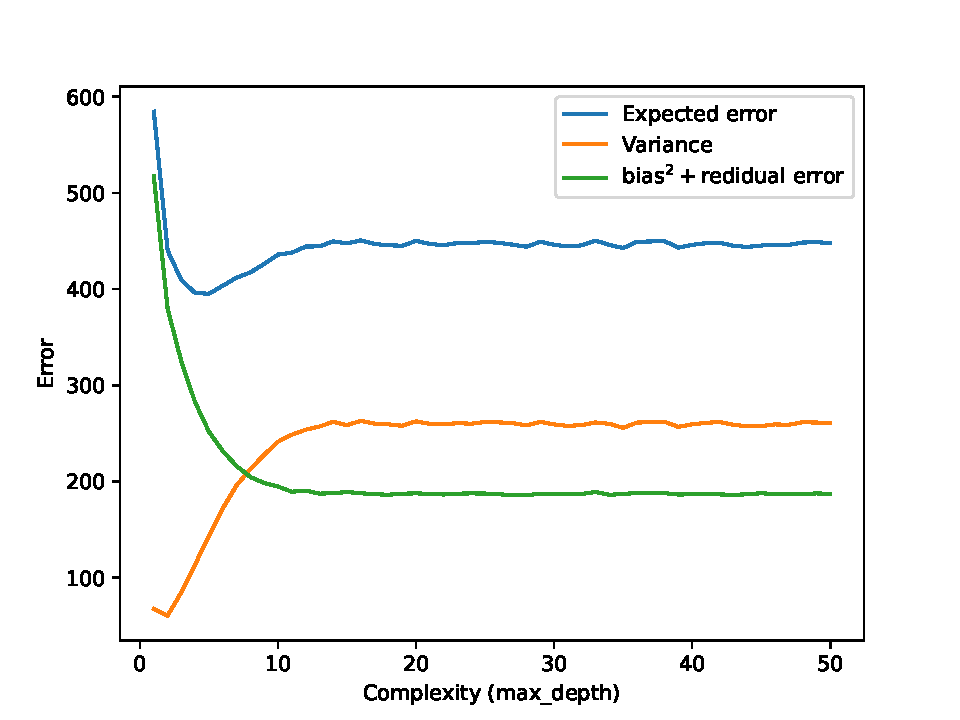
\includegraphics[scale = 0.8]{image/2.3_dt_regressor.pdf}
    \caption{Error of tree regression related to complexity}
    \label{fig:error_dt}
\end{figure}

\subsection{Impact of the size of LS on bias and variance}

\subsubsection{Ridge regression}

Ridge regression is a type of linear regression that penalizes large coefficients by adding a term proportional to their squared sum to the loss function. The complexity of ridge regression depends on the size of the learning set and the value of the penalty parameter $\alpha$ (see equation \ref{eq:loss_fct}).

In Figure~\ref{fig:ls_ridge}:
\begin{itemize}
    \item 
    For larger learning sets, the variability of the coefficients is reduced and increase the bias, while larger $\alpha$ values constrain the coefficients more and reduce the variance.
    When $\alpha$ is null, we are back with the classic linear regression whose complexity is independent from the size of the learning set. \\
    Indeed, the loss function of ridge regression, as expressed in equation (\ref{eq:loss_fct}), indicates that increasing the number of data points only increases the Residual Sum of Squares (RSS) and not the second term. This restricts the coefficients from changing significantly under fluctuations in the learning set. The set of possible $\xi$ (and hence the set of possible hyperplanes) coming from different datasets is much more limited when the number of data points is large.
\end{itemize}

\begin{figure}[H]
    \centering
    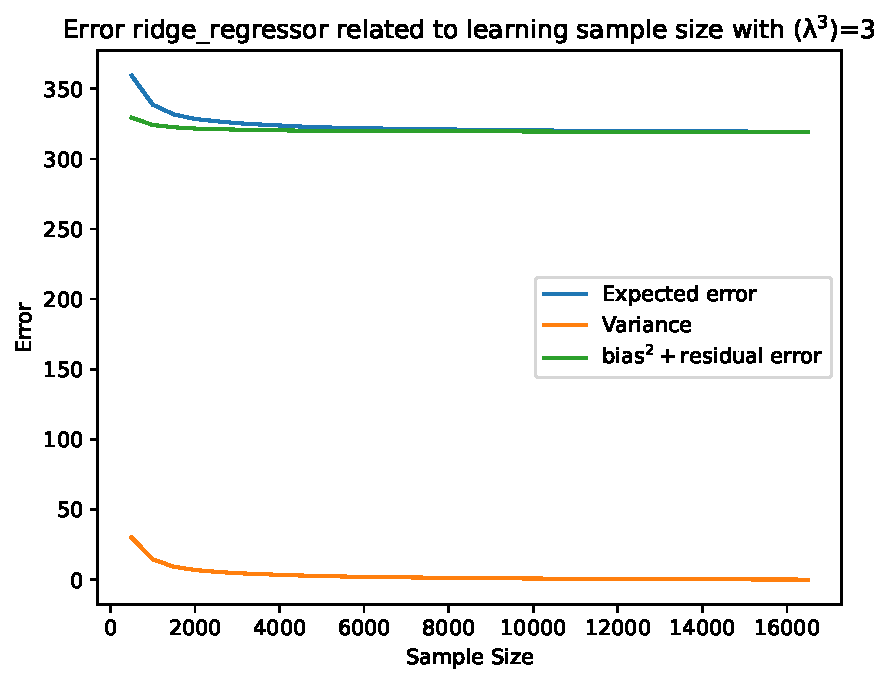
\includegraphics[scale = 0.6]{image/2.4_ridge_regressor_3-500-17000-500.pdf}
    \caption{Ridge regression model: impact of the size of the learning samples on error, variance and bias}
    \label{fig:ls_ridge}
\end{figure}

\subsubsection{k-NN}
In Figure \ref{fig:ls_knn}:
\begin{itemize}
    \item 
    The variance of a kNN model tends to decrease as the size of the learning sample increases. This is because with more data, the model has a larger pool of neighbors to choose from, which can lead to more stable and consistent predictions. However, the effect on variance also depends on the value of k. With k set to 7, the model is somewhat robust to noise in the data, but it might still be sensitive to local fluctuations in the data distribution.

    \vspace{0.3cm}

    \item 
     The bias decreases but the model complexity is fixed, it means our parameter value is poorly choose. Indeed, a fixed $k$ value means the model always considers the same number of neighbors, regardless of the size of the learning sample. When the learning sample size increases, the nearest neighbors are likely to be closer to the point chosen in the feature space, leading to more accurate predictions and lower bias.
    
\end{itemize}

\begin{figure}[H]
    \centering
    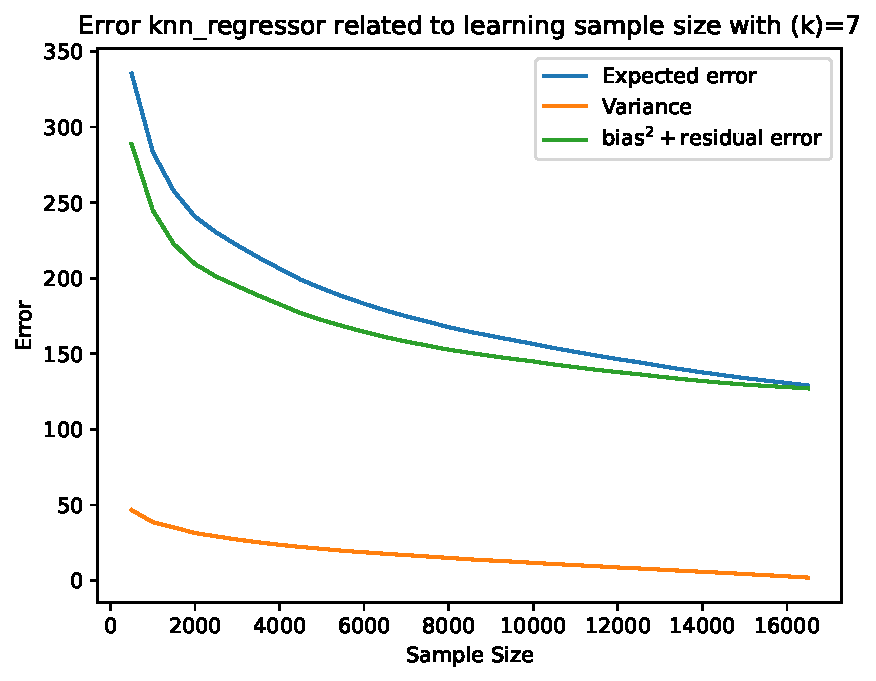
\includegraphics[scale = 0.6]{image/2.4_knn_regressor_7-500-17000-500.pdf}
    \caption{k-NN Model: impact of the size of the learning samples on error, variance and bias}
    \label{fig:ls_knn}
\end{figure}

\subsubsection{Regression trees}
The complexity of this algorithm is dependent on the size of the learning set which means we’ll observe an evolution of all the values. Indeed, it can be seen in figure \ref{fig:ls_dt} that the
bigger the learning set, the lower the values of bias, variance and expected error. 
In other words, the model get better with a bigger learning set. \\
For regression trees, two cases are possible:
\begin{itemize}
    \item 
    For fixed depths, we observe on Figure \ref{fig:ls_dt} that the bias is constant and the variance drops when increasing the leaning sample size. As explained above, in this case the complexity of the model doesn’t depend on the learning sample size. Another thing we notice is that as said in Question 2.3, when the depth increases, the variance increases and the bias decreases.

    \vspace{0.3cm}

    \item 
    For fully grown trees, the complexity depends on the learning sample size. Indeed, the depth of the tree will depend on the number of samples in the learning sample. We observe that the bias as the variance decreases with the number of LS.
\end{itemize}

\begin{figure}[H]
    \centering
    \begin{subfigure}[t]{.49\textwidth}
        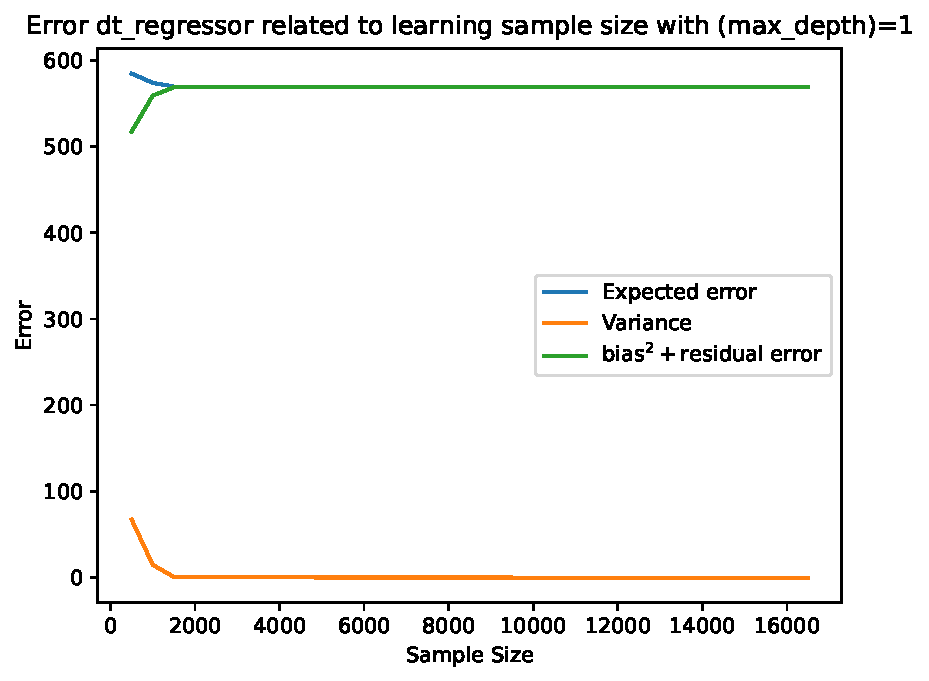
\includegraphics[width =\textwidth]{image/2.4_dt_regressor_1-500-17000-500.pdf}
        \caption{Regression tree model: $max\_depth = 1$}
        \label{fig:ls_dt_1}
    \end{subfigure}
    \hfill
    \begin{subfigure}[t]{.49\textwidth}
        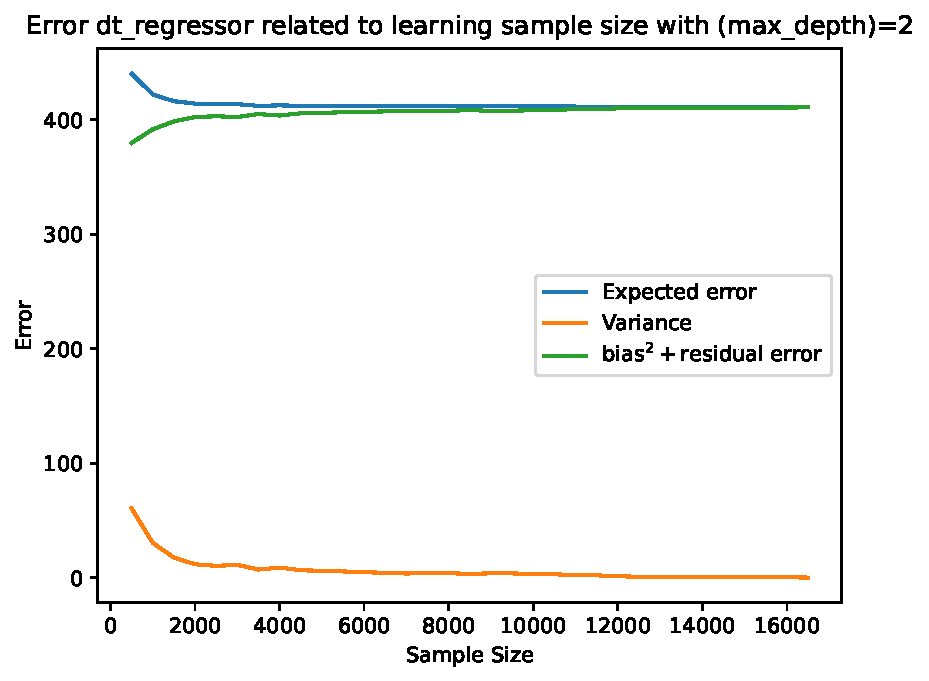
\includegraphics[width =\textwidth]{image/2.4_dt_regressor_2-500-17000-500.pdf}
        \caption{Regression tree model: $max\_depth = 2$}
        \label{fig:ls_dt_2}
    \end{subfigure}
    \hfill
    \begin{subfigure}[t]{.49\textwidth}
        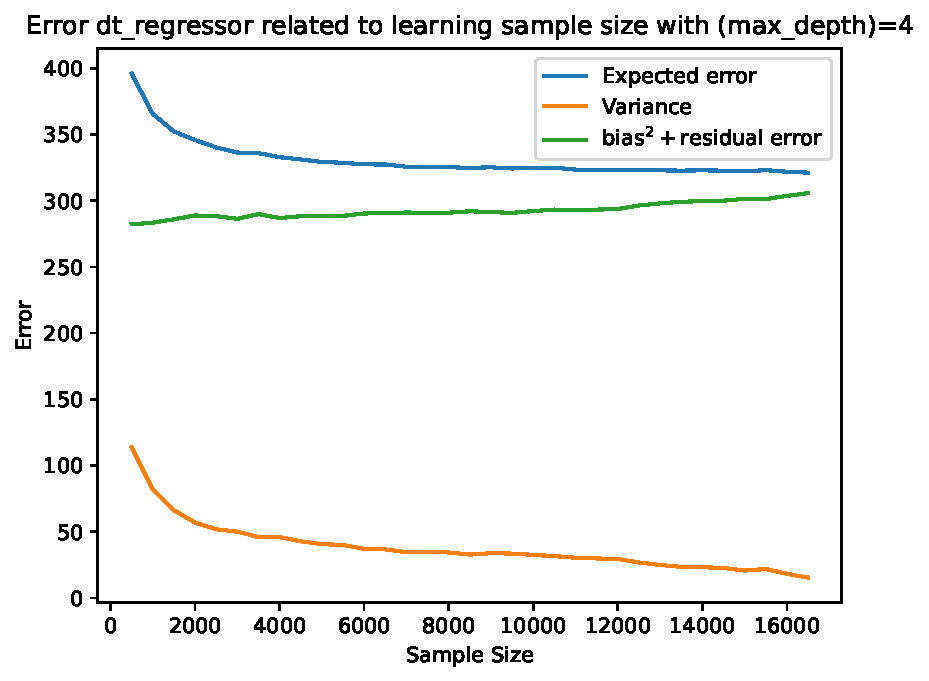
\includegraphics[width =\textwidth]{image/2.4_dt_regressor_4-500-17000-500.pdf}
        \caption{Regression tree model: $max\_depth = 4$}
        \label{fig:ls_dt_4}
    \end{subfigure}
    \hfill
    \begin{subfigure}[t]{.49\textwidth}
        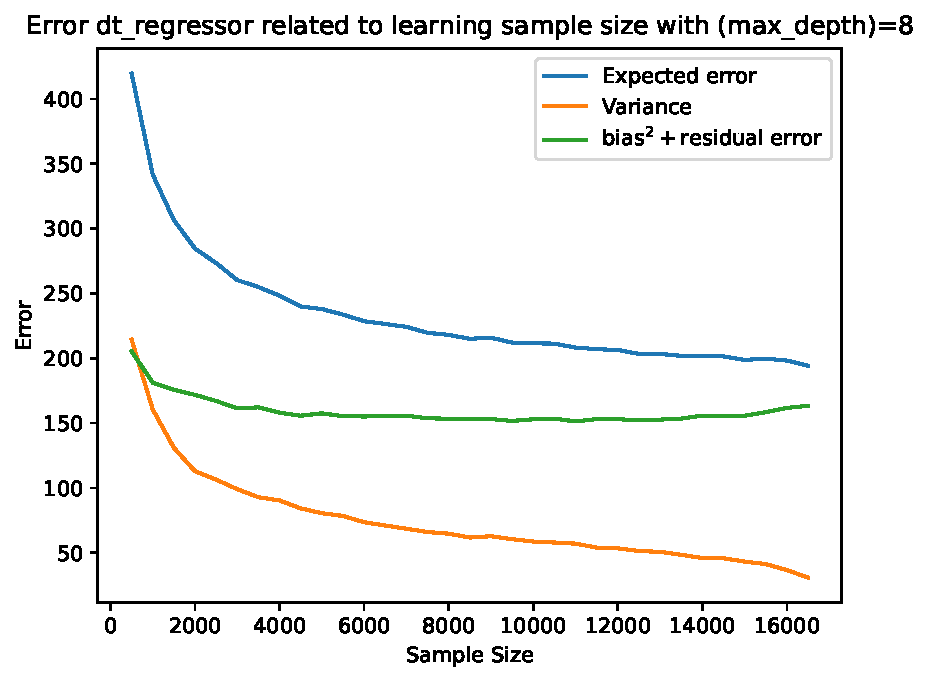
\includegraphics[width =\textwidth]{image/2.4_dt_regressor_8-500-17000-500.pdf}
        \caption{Regression tree model: $max\_depth = 8$}
        \label{fig:ls_dt_8}
    \end{subfigure}
    \caption{Error of Decision tree regressor related to learning sample size with different depth size}
    \label{fig:ls_dt}
\end{figure}

\begin{figure}[H]\ContinuedFloat
    \centering
    \begin{subfigure}[t]{.49\textwidth}
        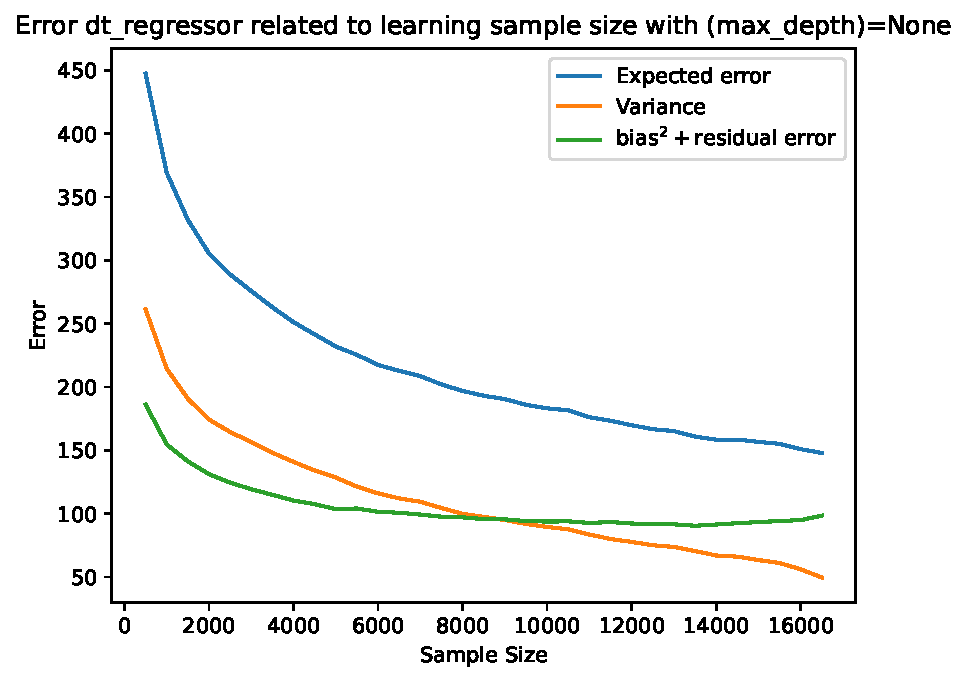
\includegraphics[width =\textwidth]{image/2.4_dt_regressor_None-500-17000-500.pdf}
        \caption{Regression tree model: $max\_depth = None$}
        \label{fig:ls_dt_none}
    \end{subfigure}
    \caption{Error of Decision tree regressor related to learning sample size with different depth size}
    \label{fig:ls_dt}
\end{figure}

\subsubsection{Conclusion}
Overall in all 3 cases,we see that when we increase the number of learning samples, the error and the variance
automatically decreases and ends up by stabilizing.

\subsection{Bootstrap aggregating (bagging method)}

Bagging, or bootstrap aggregating, is an ensemble machine learning method that involves creating multiple subsets of the original training data with replacement (bootstrap samples), training a model on each subset, and then averaging the results to form an ensemble prediction. It is particularly effective to reduce variance and improve prediction stability, often with a slight increase in bias.

We are implementing bagging with fully grown regression trees, ridge regression with $\lambda$=30 and k-Nearest Neighbors with k=1. Our approach uses 80\% of the instances for training and 20\% for testing. Here are the results obtained:

\begin{table}[H]
    \centering
    \begin{tabular}{|l|cc|cc|}
        \hline
        \textbf{Model} & \multicolumn{2}{c|}{\textbf{Bias}} & \multicolumn{2}{c|}{\textbf{Variance}} \\
        \cline{2-5}
                       & w/o Bag. & w/ Bag. & w/o Bag. & w/ Bag. \\
        \hline
        Ridge Regression & 323.2082 & 323.1924 & 838.0827 & 0.7438 \\
        \hline
        kNN              & 121.2344 & 104.4242 & 1169.0972 & 47.5971 \\
        \hline
        Regression Tree  & 141.3675 & 100.2985 & 1128.2149 & 80.1095 \\
        \hline
    \end{tabular}
    \caption{Comparison of Bias and Variance for Models With and Without Bagging}
    \label{tab:model_comparison_bagging}
\end{table}



\subsubsection{Ridge regression (with fixed $\lambda$=30)}

\begin{figure}[H]
    \centering
    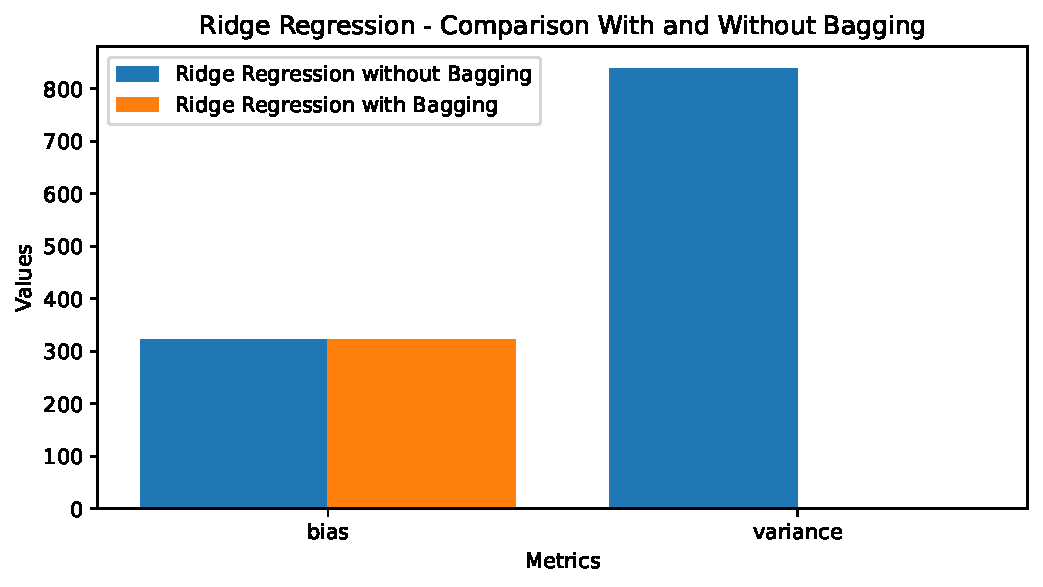
\includegraphics[scale=0.8]{image/2_5_Ridge Regression_comparison.pdf}
    \caption{Comparison of Ridge Regression Model With and Without Bagging}
    \label{fig:ridge_regression_comparison}
\end{figure}

The application of bagging on Ridge Regression showed a remarkable reduction in variance. This decrease in variance is a significant outcome considering that Ridge Regression, a regularized form of linear regression, is already designed to manage the trade-off between bias and variance. Contrary to typical expectations with bagging, the bias remained largely unaffected, indicating that the averaging effect did not introduce the slight increase in bias often associated with this technique.

\subsubsection{k-NN (w/ k=1)}

\begin{figure}[H]
    \centering
    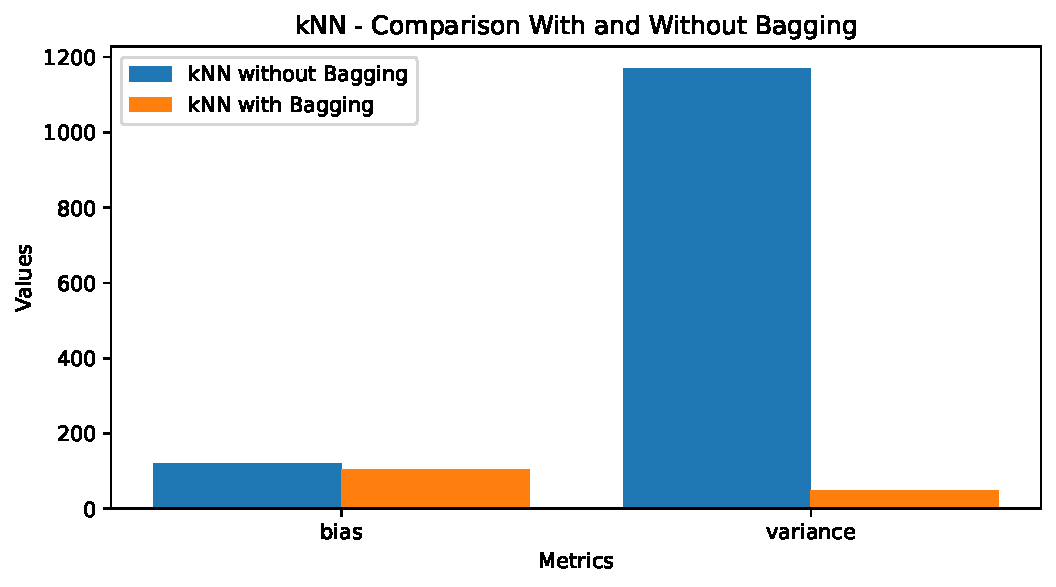
\includegraphics[scale=0.8]{image/2_5_kNN_comparison.pdf}
    \caption{Comparison of kNN Model With and Without Bagging}
    \label{fig:knn_comparison}
\end{figure}

The application of bagging on kNN significantly reduced the variance, addressing the model's tendency for high variance, especially when k=1. While there was also a reduction in bias, it was less pronounced compared to the reduction in variance. This reduction in bias might be partly attributed to the averaging effect of bagging, which can smoothen the model's sensitivity to noise in the training data.

\subsubsection{Regression trees (fully grown, w/ depth=None)}

\begin{figure}[H]
    \centering
    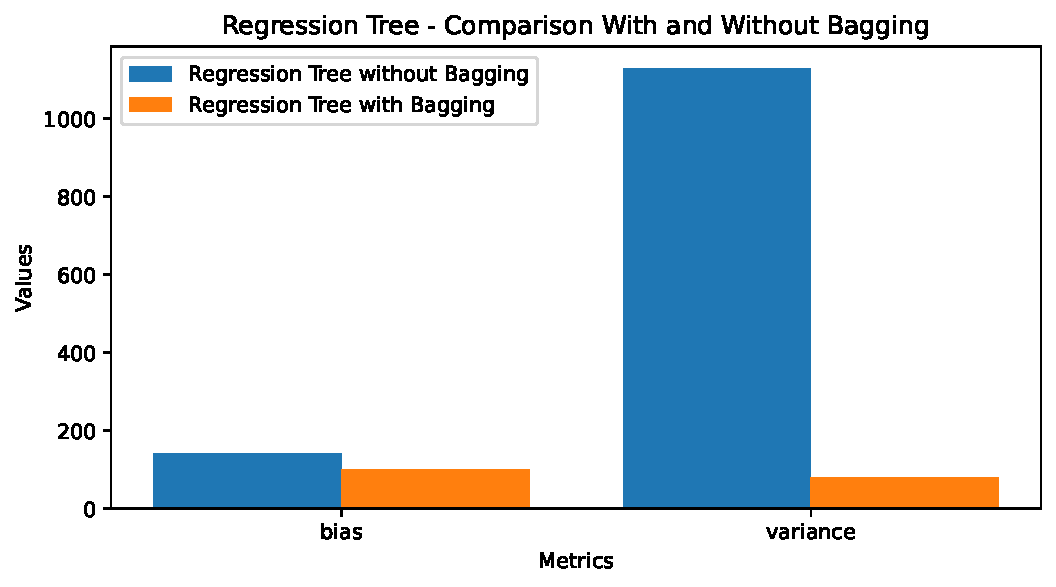
\includegraphics[scale=0.8]{image/2_5_Regression Tree_comparison.pdf}
    \caption{Comparison of Regression Tree Model With and Without Bagging}
    \label{fig:reg_tree_comparison}
\end{figure}

For Regression Trees, bagging led to a substantial reduction in variance, which is particularly important given the model's propensity for high variance due to overfitting in its fully grown state. The reduction in bias, though present, was less substantial than the reduction in variance.

\subsubsection{Conclusion}

Bagging proved to be highly effective in reducing variance across all three models. This is consistent with the theoretical understanding of bagging, which aims to reduce overfitting through averaging multiple predictions from models trained on different subsets of data.

\end{document}
